\chapter{Implementare, teste}

În aceast capitol vom prezenta aplicația, începând de la arhitectură, continuând apoi spre funcționalitatea oferită. Idea este să punem in aplicare conceptele teoretice de la capitolele anterioare, punând accent pe algoritmii de la secțiunea Aritmetica Eficienta, capitolul 2. Implementarea eficientă si corectă a acestor operații reprezintă un prim pas foarte important spre dezvoltarea de aplicații criptografice folosite în lumea reală, precum ECDSA.
\\ Pentru implementare am ales limbajul de programare Python, versiunea 3.5.2, iar hardware-ul folosit in tabelele de test este: Quad Core CPU, i7-4700HQ, 2.4 GHz, 64 bit OS, 16 GB RAM.

\section{Arhitectura Aplicației}
%arhitectura(Inclusiv grupul folosit, curbele eliptice Nist), diagrama UML cu clasele
În această aplicație s-a urmărit scrierea unui cod cât mai flexibil și concis, care să permită manipularea și aprofundarea conceptelor abstracte, matematice, discutate în secțiunile predente. Scopul final al aplicației a fost implementarea protocolul \textit{ECDSA} și un studiu comparativ al performanței algoritmilor discutati in Capitolul 2, Secțiunea Aritmetică Eficientă. \\
Deși limbajul folosit suportă atât paradigma de programare orientată pe obiecte, cât si cea procedurală, în această aplicație am ales structurarea aproape completă a codului în clase, fiecare cu roluri bine definite, pe cât posibil în concordanță cu principiile \textit{SOLID}\cite{solid}, fară însă a face compromisuri în ceea ce privește flexibilitatea si simplitatea codului. Diagrama \textit{UML}\cite{uml} din figura 4.1 surprinde toate clasele din aplicație si relațiile dintre acestea. Se observă folosirea unor clase abstracte, deși nu există suport nativ pentru ele în Python. Acestea au fost folosite pentru a reduce multe din reduntanțele care apăreau în cod și pentru a oferi un sablon pentru anumite funcționalități care pot fi introduse în aplicație. Abstractizarea claselor în Python se face cu ajutorul pachetului \textit{abcMeta}\cite{abcMeta}.\\
Funcționalitatea oferită de protocolul ECDSA, adică generarea cheilor, semnarea mesajului si verificarea semnăturii este încapsulată în 3 clase: \textit{GenerateKeyPair}, \textit{GenerateSignature}, \textit{VerifySignature}. Algoritmii care vor apărea în Studiul Comparativ sunt implementați în clasele \textit{ScalarMultiplication} și \textit{JointMultiplication}. În continuare, voi prezenta structurile de date care stau la baza aplicației.

\begin{figure}[htp]
\centering
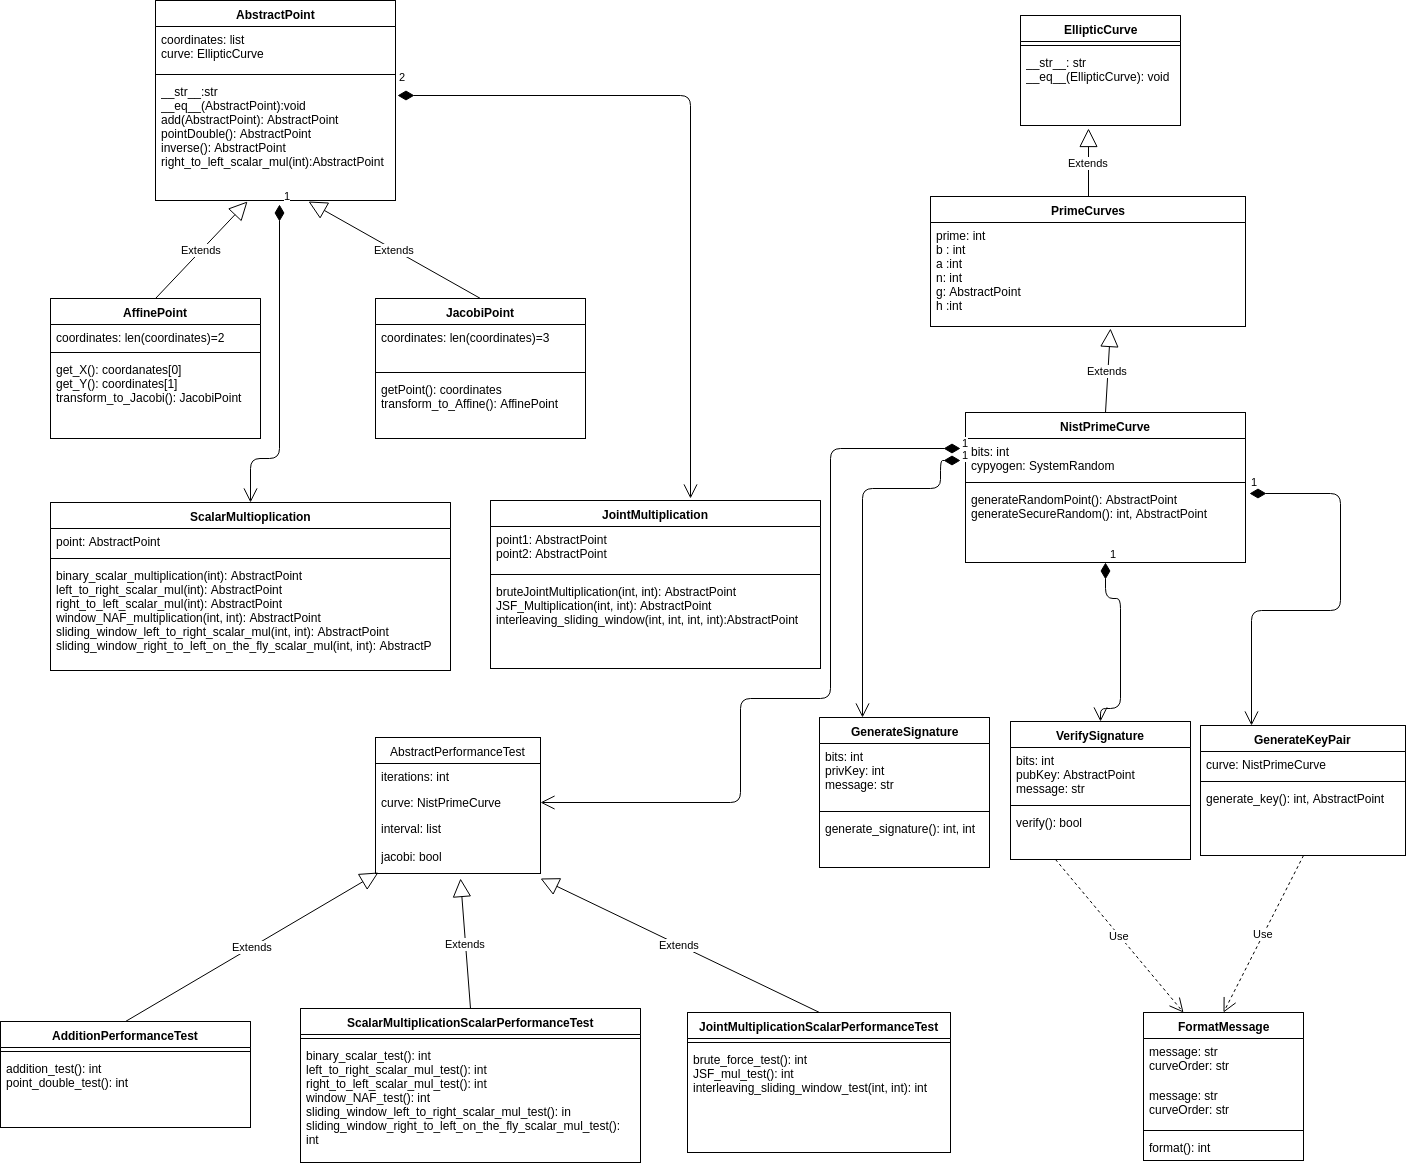
\includegraphics[width=17.5cm]{chapters/Arhitectura.png}
\caption{Arhitectura Aplicației}
\label{fig:lion}
\end{figure}

\subsection{Structuri de date}

În aplicație a fost necesară modelarea a două entități fundamentale, curba eliptică și punctul de pe o curbă eliptică. Pentru ambele concepte am creat clase abstracte, întrucât există multe tipuri de curbe eliptice, iar punctele pot avea și ele mai multe reprezentări.

\subsubsection{Curba Eliptică}
Am ales sa modelez conceptele de curbă eliptică peste un corp prim(clasa concretă \textit{PrimeCurves}) și extensia acesteia care modelează curbele NIST peste corpuri prime, \textit{NistPrimeCurve}. Clasa abstractă pentru o curbă eliptică este special modelată vag, din cauza multitudinii de tipuri de curbe existente, cu proprietăți specifice foarte speciale. Clasa \textit{PrimeCurves} modelează orice curbă definită peste un corp prim si în afara parametrilor care definesc curba si a supraîncărcării operatorilor de egalitate si de reprezentare string a obiectului, am decis să nu adaug metode speciale. Curbele Nist, definite peste corpuri prime si modelate în clasa \textit{NistPrimeCurve} au parametrii cunoscuți, definiți în \cite{nist}.

\subsubsection{Punctele de pe o curbă eliptică}

Am modelat punctele reprezentate in coordonate afine (\textit{AffinePoint}) și punctele în coordonate jacobiene (\textit{JacobiPoint}).
Design-ul punctelor a fost conceput în așa fel încat fiecare punct să conțină metode pentru operațiile de grup pentru curbe eliptice: adunare, dublare, invers. De asemenea, fiecare punct, are coordonate si aparține unei curbe, lucru reflectat în constructorul clasei \textit{AbstractPoint}. Am luat decizia să nu adaug in clasele pentru puncte metode de înmulțire cu un scalar sau de înmulțire multiplă deoarece cei mai eficienți algoritmi necesită precalcularea unor valori, acest lucru adaugând un overhead clasei punct. Astfel, cel mai eficient algoritm de înmultire a fost separat într-o clasă, care se ocupă special de această operație La fel am procedat și cu operația de înmulțire multiplă. \\

Abstractizarea acestor concepte ajută la eventuala extindere a aplicației și la evitarea codului duplicat. Prin extinderea claselor abstracte, putem adauga suport pentru alte tipuri de curbe eliptice, precum cele definite peste corpuri binare, curbe Edwards, sau suport pentru diferite tipuri de coordonate și operațiile speciale aferente.


\section{Aritmetică}
\label{subsec:subsec02}
În această secțiune vom aborda operațiile de grup pentru curbe eliptice, adunare, dublare, invers și operațiile speciale, înmulțirea cu un scalar și înmulțirea multiplă. Cele din urmă au fost explicate în capitolul doi, secțiunea Aritmetică Eficientă. Aici ne vom concentra pe implementarea acestora și rolul acestora în Studiul Comparativ, respectiv în protocolul ECDSA. \\

Justifici clasele ScalarMultiplier, zici ca prezinti  atat aritmetica de grup cat si cea speciala... 

\subsection{Operații de Grup}
În aplicatie am implementat operațiile care țin de grupul punctelor de pe o curbă eliptică în cele doua clase concrete pentru puncte, cele pentru coordonate afine si pentru coordonate jacobiene. Algoritmii de adunare constau în aplicarea unor formule, cele pentru coordonate afine fiind explicitate în Capitolul 2, Secțiunea Grupul Punctelor de pe o curba eliptică. Formulele de adunare și dublare a unui punct pentru coordonate Jacobiene sunt conform acestei surse \cite{jacobian}.

Operațiile care țin de structura de grup au o importanță deosebită, întrucât sunt folosite în fiecare algoritm de înmulțire cu scalar și implicit de înmulțire multiplă. Din acest motiv, ne dorim o implementare cât mai eficientă, orice înbunătățire la acest nivel aducând sporuri de performanță peste tot în aplicație. În coordonate afine, apare algoritmul lui Euclid Extins în calculul unor inverși modulari, astfel justificând folosirea coordonatelor jacobiene, care prin introducerea unui set de redundanțe în reprezentarea unui punct, elimină nevoia de a calcula inverși modulari. În continuare vom prezenta implementarea adunării și dublării unui punct în coordonate jacobiene. 

\begin{lstlisting}
def add(self, other):
    if self is None:
        return other
    if other is None:
        return self

    u1 = (self.x * other.z ** 2) % self.curve.prime
    u2 = (other.x * self.z ** 2) % self.curve.prime
    s1 = (self.y * other.z ** 3) % self.curve.prime
    s2 = (other.y * self.z ** 3) % self.curve.prime
    if u1 == u2:
        if s1 != s2:
            return None
        else:
            return self.point_double()

    h = (u2 - u1) % self.curve.prime
    r = (s2 - s1) % self.curve.prime
    x3 = (r ** 2 - h ** 3 - 2 * u1 * h ** 2) % self.curve.prime
    y3 = (r * (u1 * h ** 2 - x3) - s1 * h ** 3) % self.curve.prime
    z3 = (h * self.z * other.z) % self.curve.prime
    return Jacobi_Point([x3, y3, z3, pow(z3, 2, self.curve.prime), 
           pow(z3, 3, self.curve.prime)], self.curve)
\end{lstlisting}

\begin{lstlisting}
def point_double(self):
    if self is None:
        return None
    if self.y == 0:
        return None
    s = (4 * self.x * self.y ** 2) % self.curve.prime
    m = (3 * self.x ** 2 + self.curve.a * self.z ** 4) % self.curve.prime
    _x = (m ** 2 - 2 * s) % self.curve.prime
    _y = (m * (s - _x) - 8 * self.y ** 4) % self.curve.prime
    _z = (2 * self.y * self.z) % self.curve.prime
    return Jacobi_Point([_x, _y, _z, pow(_z, 2, self.curve.prime), 
	   pow(_z, 3, self.curve.prime)], self.curve)
\end{lstlisting}

Atât în coordonate afine, cât și în cele jacobiene, inversul unui punct este foarte simplu de calculat, prin negarea componentei a doua din reprezentarea punctului. Singurul dezavantaj al folosirii coordonatelor jacobiene îl constituie operația de trecere înapoi în coordonate afine, operație care necesită calcului a doi inverși modulari.

\begin{lstlisting}
def transform_to_affine(self):
       return AffinePoint([self.coordinates[0] * inv(self.coordinates[2] ** 2, 	    self.curve.prime) % self.curve.prime, (self.coordinates[1] * inv(self.coordinates[2] ** 3  3, self.curve.prime)) % self.curve.prime], self.curve)
\end{lstlisting}

\subsection{Înmulțirea cu un scalar}

Putem aborda problema înmulțirii cu un scalar în diferite feluri, de la cele mai ineficiente metode(apelararea functiei de adunare de cate ori este nevoie) până la metode sofisticate și eficiente, cum ar fi înmulțirea cu fereastră glisantă.

\subsubsection{Metoda Binară}

Prima metodă pe care am implementat-o este cea binară. Algoritmul constă în procesarea reprezentării binare a scalarului de la cel mai nesimnificativ bit la cel mai semnificativ.

\begin{lstlisting}
def binary_scalar_multiplication(self, d):
    P = self.point
    if d == 0:
        return None
    if d == 1:
        return P
    result = None
    while d > 0:
        if d % 2:
            result = P.add(result)
        d //= 2
        P = P.add(P)
    return result
\end{lstlisting}

În variabila \textit{result}, ținem rezultatul după fiecare iterație, iar în variabila $P$ ținem o copie punctului care dorim să îl înmulțim. Astfel, după fiecare bit parcurs dublăm $P$ și când întâlnim un bit de $1$ adunăm la rezultat $P$. La final returnăm variabila \textit{result}.

\subsubsection{Reprezentări cu semn}

Un avantaj major al grupului punctelor de pe o curbă eliptică îl reprezintă calculul foarte ușor din punct de vedere computațional al inversului. Astfel, putem să apelăm la reprezentările cu semn pentru scalar, acestea optimizând calculul de înmulțire cu un scalar. Cea mai eficientă astfel de reprezentare este $NAF$. \\

În continuare voi prezenta un algoritm pentru calculul reprezentării $NAF$. \\

\begin{lstlisting}
def naf(d):
    i = 0
    res = []
    while d >= 1:
        if d % 2 == 0:
            res.append(0)
        else:
            res.append(2 - d % 4)
            d -= res[i]
        d //= 2
        i += 1
    return res[::-1]
\end{lstlisting}

Cifrele care formează reprezentarea  $NAF$ sunt generate de resturile împărțirii repetate a scalarului la $2$. Această împărțire este una cu semn, resturile putând fii $\set{0, 1, -1}$. Când, în bucla \textit{while}, scalarul $d$ este impar și trebuie sa alegem între $r\in\set{-1, 1}$, alegem în așa fel încât $\frac{d-r}{2}$ să fie par, astfel făcând ca următoarea cifră din $NAF$ să fie $0$.

Având la dispoziție metoda pentru aflarea reprezentării cu semn a unui numar natural, putem eficientiza metoda binară. Algoritmul de la stânga la dreapta pentru calculul lui $dP$, unde d este scalarul si $P$ este un punct de pe o curba eliptica, apelează funcția pentru reprezentare cu semn. Parcurgem aceasta, dublând cantitatea din variabila \textit{result} după fiecare bit parcurs, iar la bitul de 1 adunăm punctul $P$, la bitul $-1$ scadem $P$ din rezultat. Urmează implementarea acestui algoritm.

\begin{lstlisting}
def left_to_right_scalar_mul(self, d):
    signed_d = naf(d)
    result = None
    for i in signed_d:
        if result is None:
            result = None
        else:
            result = result.point_double()
        if i == 1:
            result = self.point.add(result)
        if i == -1:
            result = self.point.inverse().add(result)
    return result
\end{lstlisting}

Algoritmul de la dreapta la stânga funcționează în același mod, singura diferență fiind faptul că NAF-ul este calculat în aceași buclă while în care calculăm rezultatul final. În acea buclă descompunem scalarul, ținem bit-ul curent într-o variabilă, $u$, iar apoi în funcție de valoarea acestuia modificăm rezultatul. Cei doi algoritmi au aceași complexitate asimtotică.

\begin{lstlisting}
def right_to_left_scalar_mul(self, d):
    result = None
    R = self.point
    while d >= 1:
        if d % 2 == 1:
            u = 2 - (d % 4)
            d -= u
            if u == 1:
                result = R.add(result)
            else:
                result = R.inverse().add(result)
        d //= 2
        R = R.point_double()
    return result
\end{lstlisting}

\subsubsection{Metoda cu fereastră}

Metoda cu fereastră poate fi privită ca o generalizare a metodei cu semn, aceasta aducând plusuri de performanță în schimbul folosirii unui plus de memorie. Această metodă se folosește de reprezentarea $w-NAF$ a scalarului.
Un algoritm eficient pentru calculul $w-NAF$ va fi prezentat în continuare. Funcția mods este modulo cu semn, adica pentru un scalar $d$, avem $d$ mods $2^w=u$, unde u este un numar intreg care satisface $u\equiv d$ mod $2^w$ si $-2^{w-1}\leq u\leq 2^{w-1}$.

\begin{lstlisting}
def w_NAF(d, w):
    i = 0
    res = []
    while d >= 1:
        if d % 2 == 0:
            res.append(0)
        else:
            res.append(mods(d, w))
            d -= res[i]
        d //= 2
        i += 1
    return res[::-1]
\end{lstlisting}

Se observă că cifrele din $w-NAF$ sunt de fapt restul împărțirii cu semn a scalarului la $2$, rest care aparține intervalului $[-2^{w-1}, 2^{w-1}-1]$. Astfel, daca scalarul $d$ este impar și $r = d$ mods $2^w$, atunci $\frac{d-r}{2}$ este divizibil cu $2^{w-1}$, asigurând astfel ca următoarele $w-1$ cifre din reprezentare sunt $0$.
 
Metoda cu fereastră aduce un plus de performanță prin reducerea numărului de adunări necesare în calculul multiplului unui punct oarecare $P$ de pe o curbă eliptică. Aici vom folosi reprezentarea $w-NAF$ in loc de $NAF$. Vom precalcula și stoca valorile pentru $iP$ si $i\in\set{1, 2^{w-1}}$. Astfel, când parcurgem $w-NAF$ -ul numarului, în funcție de cifra gasită vom aduna sau scădea din rezultat valorile potrivite din multimea de valori precalculate, dublând variabila acumulator la fiecare iterație.

\begin{lstlisting}
def window_NAF_multiplication(self, d, w):
    d = w_NAF(d, w)
    Q = None
    for i in range(0, len(d)):
        if Q is None:
            Q = None
        else:
            Q = Q.point_double()
        if d[i] != 0:
            if d[i] > 0:
                Q = P[d[i]].add(Q)
            else:
                Q = P[-d[i]].inverse().add(Q)
    return Q
\end{lstlisting}

Valorile precalculate sunt stocate într-un dicționar \textit{P}. Dicționarul în Python este o structură de date de tip \textit{Hash Map}. Am ales să stochez astfel, din cauză că această structură de date oferă lookup-uri foarte rapide, în $\mathcal{O}(1)$ amortizat.

O versiune ușor modificată a algoritmului precedent este propusă în \cite{sliding2}. Acesta este un algoritm de la dreapta la stânga, care calculează $w-NAF$ pentru scalar în aceași buclă în care este calculat și rezultatul. Valorile diferite de zero din reprezentare sunt stocate intr-un Hash Map si rezultatul este calculat la final, prin adunarea valorilor stocate și returnat.

\begin{lstlisting}
def window_NAF_on_the_fly_scalar_mul(self, k, w):
    R = self.point
    m = 2**(w-1) - 1
    Q = {}
    for i in range(1, m + 1, 2):
        Q[i] = None
    while k >= 1:
        if k % 2 == 1:
            t = mods(k, w)
            if t > 0:
                Q[t] = R.add(Q[t])
            if t < 0:
                Q[-t] = R.inverse().add(Q[-t])
            k -= t
        R = R.point_double()
        k //= 2
    for i in range(3, m + 1, 2):
        if Q[i] is not None:
            Q[1] = Q[i].right_to_left_scalar_mul(i).add(Q[1])
    return Q[1]
\end{lstlisting}.

\subsubsection{Metoda cu fereastră glisantă}

Diferența dintre metoda prezentată anterior și aceasta constă în faptul că aceasta din urmă ne permite să sărim peste zerourile din reprezentarea $w-NAF$ a scalarului. Pentru această metodă vom implementa o versiune ușor modificată față de cea originală, propusă de către \cite{sliding}.

Algoritmul apelează funcția pentru $w-NAF$ si parcurge în bucla while această reprezentare. Când găsim prima cifră diferită de zero, o procesăm, adăugam la rezultat valoarea corespunzătoare din dicționarul de valori precalculate, apoi "glisăm" fereastra peste cifrele care sunt zero.

\begin{lstlisting}
def sliding_window_left_to_right_scalar_mul(self, d, w):
    d = w_NAF(d, w)
    Q = None
    i = 0
    while i < len(d):
        if d[i] == 0:
            if Q is None:
                Q = None
            else:
                Q = Q.point_double()
            i += 1
        else:
            s = max(len(d) - i - w + 1, 0)
            s = len(d) - 1 - s
            while d[s] == 0:
                s -= 1
            u = NAF(d[i:s + 1])
            for j in range(1, i - s + 2):
                if Q is not None:
                    Q = Q.point_double()
                else:
                    Q = None
            if u > 0:
                Q = _P[u].add(Q)
            if u < 0:
                Q = Q.add(_P[-u].inverse())
            i = 1 + s
    return Q
\end{lstlisting}

\subsection{Înmulțirea multiplă}
\label{subsec:subsec04}

\subsection{Metoda Naivă}

\begin{lstlisting}
def brute_joint_multiplication(self, k, l):
    result1 = self.multiplier1.sliding_window_left_to_right_scalar_mul(k)
    result2 = self.multiplier2.sliding_window_left_to_right_scalar_mul(l)
    return result1.add(result2)
\end{lstlisting}

\subsubsection{Metoda cu Joint Sparse Form}

\begin{lstlisting}
def JSF_Multiplication(self, k, l):
    """Add using Shamir Trick, variation of algorithm 3.48, Menezez Book"""
    jsf = self.JSF(k, l)
    assert len(jsf[0]) == len(jsf[1])

    P = self.point1
    Q = self.point2

    R = None

    precom = (
              (None, Q, Q.inverse()),
              (P, P.add(Q), P.add(Q.inverse())),
              (P.inverse(), Q.add(P.inverse()), P.inverse().add(Q.inverse()))
    )

    for i, j in zip(jsf[0], jsf[1]):
        if R is None:
            R = None
        else:
            R = R.point_double()
        if i or j:
            R = precom[i][j].add(R)
        return R
\end{lstlisting}

\subsubsection{Metoda cu fereastră glisantă intercalată}

\begin{lstlisting}
def interleaving_sliding_window(self, k, l, w1, w2):
    """Algorithm 3.5.1 menezez, 'Interleaving with NAF' """

    _P = {}
    _Q = {}
    R = None
    naf = [w_NAF(k, w1), w_NAF(l, w2)]
    _l = max([len(naf[0]), len(naf[1])])

    #precom stage
    for i in range(1, 2**(w1 - 1), 2):
        _P[i] = self.point1.right_to_left_scalar_mul(i)
    for j in range(1, 2**(w2 - 1), 2):
        _Q[j] = self.point2.right_to_left_scalar_mul(j)
 
    #padding stage
    for i in range(_l - len(naf[0])):
        naf[0].insert(i, 0)
    for i in range(_l - len(naf[1])):
        naf[1].insert(i, 0)

    for i in range(_l):
       if R is None:
            R = None
       else:
            R = R.point_double()
       for j in range(2):
            if naf[j][i] != 0:
               if naf[j][i] > 0:
                   if j == 0:
                        R = _P[naf[j][i]].add(R)
                    else:
                        R = _Q[naf[j][i]].add(R)
               else:
                    if j == 0:
                        R = _P[-naf[j][i]].inverse().add(R)
                    else:
                        R = _Q[-naf[j][i]].inverse().add(R)
    return R

\end{lstlisting}

\section{ECDSA}

\section{Eficiența implementării, Studiu Comparativ}

Nu uita sa faci un tabel cu ECDSA, eficient/ineficient... 


In continuare, vom face o comparatie intre cele doua metode de adunare, cea cu coordonate afine si cea in coordonate Jacobiene. In teste am am generat random doua numere pe o curba eliptica si le-am adunat. Am cronometrat 1000 de iteratii la fiecare test. Se poate observa per total ca adunarea in coordonate Jacobiene este de doua ori mai rapida decat cea in coordonate afine.

\begin{tabular}{ |p{3cm}||p{3cm}|p{3cm}|p{3cm}|  }
 \hline
 \multicolumn{4}{|c|}{Adunarea punctelor de pe curbe eliptice} \\
 \hline
 Curba NIST& Coordonate &Metoda &Timp de executie(secunde)\\
 \hline
 P192   & Afine    &Adunare& 5.22\\
 P192&Afine  & Dublare & 5.19\\
 P192 &Jacobiene & Adunare& 2.6\\
 P192&Jacobiene & Dublare & 2.61\\
 P224& Afine & Adunare & 6.66\\
 P224& Jacobiene & Adunare   &3.32\\
 P256& Afine  & Adunare& 8.47\\
 P256& Jacobiene  & Adunare& 4.52\\
 P384& Afine  & Adunare& 18.06\\
 P384& Jacobiene  & Adunare& 8.96\\
 \hline
\end{tabular}

Pentru teste am decis sa aleg diferite intervale pentru marimea scalarului. Pentru fiecare test sunt rulate 1000 de iteratii cu scalari alesi random in intervalul $5-32$ biti respectiv $128-198$ si $300-384$ pentru curbele $P192$ si respectiv $P384$. Se observa eficienta metodelor cu fereastra pentru numere mari, algoritmul de inmultire care foloseste reprezentarea cu semn fiind foarte eficient pentru numere mici. De asemenea nu se observa o inbunatatirea a eficientei algoritmilor daca procesam de la stanga la dreapta sau de la dreapta la stanga sau la fereastra glisanta, cand facem calculul $w-NAF$-ului in aceasi bucla while in care calculam rezultatul.

Pentru scalari mari, cele mai bune rezultate au fost obtinute cu o fereastra glisanta de latime 4, algoritmul pierzand din eficienta pentru ferestre de latime mai mare din cauza costului mare din punct de vedere computational al precalculului. 

De asemenea putem observa beneficiul impresionant adus de folosirea coordonatelor Jacobiene, acestea aducand inbunatatiri consistente de performanta, algoritmii fiind de aproximativ cinci ori mai rapizi in aceste coordonate. 


\begin{tabular}{ |p{5cm}||p{3cm}|p{3cm}|p{2cm}|p{1cm}|  }
 \hline
 \multicolumn{5}{|c|}{Curba P192} \\
 \hline
 Algoritm& Coordonate &Intervalul &Fereastra &Timp\\
 \hline
 Alg Binar & Afine  &$[2^{5},2^{32}]$& - & 2.48\\
 Alg Binar&Jacobiene  & $[2^{5},2^{32}]$ & - & 0.6\\
 Alg Binar&Jacobiene  & $[2^{128},2^{192}]$ & - & 3.88\\
 Inmultire de st. la dr. & Jacobian & $[2^{5},2^{32}]$& - & 0.39\\
 Inmultire de st. la dr. & Afine & $[2^{128},2^{192}]$& - & 14.04\\
 Inmultire de st. la dr. & Jacobian & $[2^{128},2^{192}]$& - & 2.49\\
 Inmultire de dr. la st. &Afine & $[2^{128},2^{192}]$ & - & 14.33\\
 Inmultire de dr. la st. &Jacobiene & $[2^{5},2^{32}]$ & - & 0.41\\
 Inmultire de dr. la st. &Jacobiene & $[2^{128},2^{192}]$ & - & 2.52\\
 Metoda cu fereastra& Jacobiene & $[2^{5},2^{32}]$ & 3 & 0.42\\
 Metoda cu fereastra& Jacobiene & $[2^{128},2^{192}]$ & 3 & 2.38\\
 Metoda cu fereastra& Jacobiene & $[2^{128},2^{192}]$ & 4 & 2.32\\
 Fereastra glisanta st. la dr.& Jacobiene  & $[2^{5},2^{32}]$& 3 & 0.51\\
 Fereastra glisanta st. la dr.& Jacobiene  & $[2^{128},2^{192}]$& 3 & 2.68\\
  Fereastra glisanta st. la dr.& Jacobiene  & $[2^{128},2^{192}]$& 4 & 2.04\\
 Fereastra glisanta dr. la st.& Jacobiene  & $[2^{128},2^{192}]$& 3 & 2.47\\
 Fereastra glisanta dr. la st.& Jacobiene  & $[2^{128},2^{192}]$& 4 & 2.41\\
 Fereastra glisanta dr. la st.& Jacobiene  & $[2^{128},2^{192}]$& 5 & 2.58\\
 \hline
\end{tabular}

\begin{tabular}{ |p{5cm}||p{3cm}|p{3cm}|p{2cm}|p{1cm}|  }
 \hline
 \multicolumn{5}{|c|}{Curba P384} \\
 \hline
 Algoritm& Coordonate &Intervalul &Fereastra &Timp\\
 \hline
 Alg Binar & Afine  &$[2^{5},2^{32}]$& - & 5.5\\
 Alg Binar&Jacobiene  & $[2^{5},2^{32}]$ & - & 1.12\\
 Alg Binar&Jacobiene  & $[2^{300},2^{384}]$ & - & 13.98\\
 Inmultire de st. la dr. & Jacobian & $[2^{5},2^{32}]$& - & 0.66\\
 Inmultire de st. la dr. & Afine & $[2^{300},2^{384}]$& - & 59.62\\
 Inmultire de st. la dr. & Jacobian & $[2^{128},2^{192}]$& - & 8.33\\
 Inmultire de dr. la st. &Afine & $[2^{300},2^{384}]$ & - & 59.58\\
 Inmultire de dr. la st. &Jacobiene & $[2^{5},2^{32}]$ & - & 0.69\\
 Inmultire de dr. la st. &Jacobiene & $[2^{300},2^{384}]$ & - & 8.69\\
 Metoda cu fereastra& Jacobiene & $[2^{5},2^{32}]$ & 3 & 0.68\\
 Metoda cu fereastra& Jacobiene & $[2^{300},2^{384}]$ & 3 & 8.2\\
 Metoda cu fereastra& Jacobiene & $[2^{300},2^{384}]$ & 4 & 7.89\\
 Fereastra glisanta st. la dr.& Jacobiene  & $[2^{5},2^{32}]$& 3 & 0.85\\
 Fereastra glisanta st. la dr.& Jacobiene  & $[2^{300},2^{384}]$& 3 & 8.73\\
  Fereastra glisanta st. la dr.& Jacobiene  & $[2^{300},2^{384}]$& 4 & 6.46\\
 Fereastra glisanta dr. la st.& Jacobiene  & $[2^{300},2^{384}]$& 3 & 8.17\\
 Fereastra glisanta dr. la st.& Jacobiene  & $[2^{300},2^{384}]$& 4 & 7.93\\
 Fereastra glisanta dr. la st.& Jacobiene  & $[2^{300},2^{384}]$& 5 & 8.33\\
 \hline
\end{tabular}	

\begin{tabular}{ |p{5cm}||p{3cm}|p{3cm}|p{2cm}|p{1cm}|  }
 \hline
 \multicolumn{5}{|c|}{Curba P192} \\
 \hline
  Algoritm& Coordonate &Intervalul &Ferestre &Timp\\
 \hline
 Alg Brut & Afine  &$[2^{5},2^{32}]$& - & 4.85\\
 Alg Brut & Afine  &$[2^{128},2^{198}]$& - & 26.18 \\
 Alg Brut & Jacobiene  &$[2^{5},2^{32}]$& - & 1.04 \\
 Alg Brut & Jacobiene  &$[2^{128},2^{198}]$& - & 4.89 \\
 Inmultire cu JSF & Afine  &$[2^{5},2^{32}]$& - & 2.72 \\
 Inmultire cu JSF & Jacobiene  &$[2^{5},2^{32}]$& - & 0.56 \\
 Inmultire cu JSF & Jacobiene  &$[2^{128},2^{198}]$& - & 2.35 \\
 Interleaving & Jacobiene  &$[2^{5},2^{32}]$& 3, 4 & 0.66 \\
 Interleaving & Jacobiene  &$[2^{128},2^{198}]$& 3, 3 & 3.39\\
 Interleaving & Jacobiene  &$[2^{128},2^{198}]$& 3, 4 &  3.29\\
 Interleaving & Jacobiene  &$[2^{128},2^{198}]$& 4, 4 & 3.15 \\
 Interleaving & Jacobiene  &$[2^{128},2^{198}]$& 4, 5 & 3.4 \\
 Interleaving & Jacobiene  &$[2^{128},2^{198}]$& 5, 5 & 3.55 \\
 \hline
\end{tabular}

\begin{tabular}{ |p{5cm}||p{3cm}|p{3cm}|p{2cm}|p{1cm}|  }
 \hline
 \multicolumn{5}{|c|}{Curba P384} \\
  \hline
  Algoritm& Coordonate &Intervalul &Ferestre &Timp\\
 \hline
 Alg Brut & Afine  &$[2^{5},2^{32}]$& - & 10.81\\
 Alg Brut & Afine  &$[2^{128},2^{198}]$& - & 54.17 \\
 Alg Brut & Jacobiene  &$[2^{5},2^{32}]$& - & 1.69 \\
 Alg Brut & Jacobiene  &$[2^{128},2^{198}]$& - & 8.25 \\
 Inmultire cu JSF & Afine  &$[2^{5},2^{32}]$& - & 5.92 \\
 Inmultire cu JSF & Jacobiene  &$[2^{5},2^{32}]$& - & 0.9 \\
 Inmultire cu JSF & Jacobiene  &$[2^{128},2^{198}]$& - & 3.84\\
 Interleaving & Jacobiene  &$[2^{5},2^{32}]$& 3, 4 & 1.09 \\
 Interleaving & Jacobiene  &$[2^{128},2^{198}]$& 3, 3 & 5.31 \\
 Interleaving & Jacobiene  &$[2^{128},2^{198}]$& 3, 4 & 5.41 \\
 Interleaving & Jacobiene  &$[2^{128},2^{198}]$& 4, 4 & 5.23 \\
 Interleaving & Jacobiene  &$[2^{128},2^{198}]$& 4, 5 & 5.61 \\
 Interleaving & Jacobiene  &$[2^{128},2^{198}]$& 5, 5 & 5.83	 \\
 \hline
\end{tabular}

\section{Testare}
Unit teste, sper sa am timp.. 